Один из многих возможных способов достигнуть стоимости, составляющей $77$ изюминок такой:

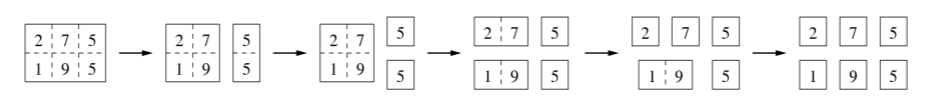
\includegraphics[scale=0.5]{raisins2.png}

Первый разрез, который Бонни просит сделать Петра, разделяет третий столбец от оставшейся
части плитки шоколада. Бонни должна заплатить за это Петру $29$ изюминок.

Затем Бонни даёт Петру меньшую из двух частей~--- ту, которая состоит из двух кусочков по $5$ изюминок в каждом, и просит Петра разрезать эту часть на две в обмен на $10$ изюминок. После этого, Бонни даёт Петру большую оставшуюся часть, в которой остались кусочки с $2$, $7$, $1$ и $9$.

изюминками соответственно. Бонни просит Петра разрезать её по горизонтали, отделяя первую
строку от второй, и платит $19$ изюминок.


После этого Бонни просит Петра разрезать левую верхнюю часть, платя $9$ изюминок. Наконец,
Бонни просит Петра разрезать левую нижнюю часть, платя $10$ изюминок.

Общая стоимость составляет $29 + 10 + 19 + 9 + 10 = 77$ изюминок. Не существует способа разрезать эту плитку шоколада на составляющие её $6$ кусочков за меньшую стоимость.